%\subsection{Ejercicio 5 - Dos páginas}\label{subsec:ej3}

Para que se generen dos páginas se hacen dos llamadas a \textit{showpage}: una al finalizar la tabla y otra al terminar la gráfica.\\

Lo primero es colocar el título, indicando posición y tipografía:
\begin{lstlisting}[language=PostScript, caption=Titulo primera página, captionpos=b, label=fun:titulo]
/Times-Bold findfont 24 scalefont setfont
newpath
    200 700 moveto
    (Mi tabla de datos: Ventas) show
\end{lstlisting}

Para simular la tabla se dibuja una cuadricula:
\begin{lstlisting}[language=PostScript, caption=Cuadricula de la tabla, captionpos=b, label=fun:tabla]
newpath
    % Líneas horizontales
    150 650 moveto 400 650 lineto
    150 620 moveto 400 620 lineto
    150 500 moveto 400 500 lineto
    
    % Líneas verticales
    150 650 moveto 150 500 lineto
    275 650 moveto 275 500 lineto
    400 650 moveto 400 500 lineto
    
    2 setlinewidth 
    0 0 0 setrgbcolor % Negro
stroke
\end{lstlisting}

Con el comando \textit{show} se coloca el texto en la tabla, con el siguiente tipo de letra:
\begin{lstlisting}[language=PostScript, caption=Tipo de fuente, captionpos=b, label=fun:tipo]
/Times-Roman findfont 16 scalefont setfont
\end{lstlisting}

La tabla se rellena con el siguiente contenido:
\begin{lstlisting}[language=PostScript, caption=Relleno de la tabla, captionpos=b, label=fun:relleno]
% Cabeceras
newpath 170 630 moveto (Mes) show
newpath 300 630 moveto (Ventas) show

% Datos inventados
newpath 170 590 moveto (Enero) show
newpath 300 590 moveto (10) show

newpath 170 550 moveto (Febrero) show
newpath 300 550 moveto (50) show

newpath 170 510 moveto (Marzo) show
newpath 300 510 moveto (20) show
\end{lstlisting}

A continuación se muestra la imagen obtenida para la primera página \myref{fig:5ejer1}:
\begin{figure}[H]
    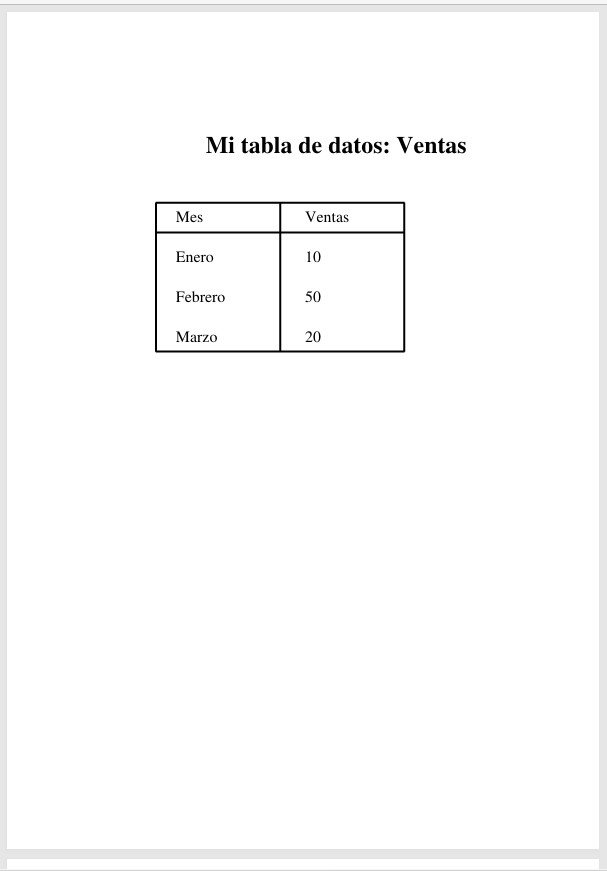
\includegraphics[width=0.9\linewidth]{images/ejer5_pg1.jpg}
    \caption{Propuesta ejercicio 5. Página 1.}
    \label{fig:5ejer1}
\end{figure}

Para dibujar la gráfica primero se pintan los ejes:
\begin{lstlisting}[language=PostScript, caption=Ejes de la gráfica, captionpos=b, label=fun:ejes]
newpath
    % Eje Y (Vertical)
    150 400 moveto
    150 600 lineto 
    
    % Eje X (Horizontal)
    150 400 moveto
    450 400 lineto 
    
    3 setlinewidth 
    0 0 0 setrgbcolor % Negro
stroke
\end{lstlisting}

Dibujo los datos en color rojo:
\begin{lstlisting}[language=PostScript, caption=Gráfica, captionpos=b, label=fun:grafica]
newpath
    150 400 moveto     % Origen
    200 450 lineto     % Sube a 10 (Enero)
    300 580 lineto     % Pico máximo de 50 (Febrero)
    400 480 lineto     % Baja a 20 (Marzo)
    
    2 setlinewidth
    1 0 0 setrgbcolor  % Color rojo
stroke
\end{lstlisting}

Por último, dibujar las etiquetas de los ejes:
\begin{lstlisting}[language=PostScript, caption=Etiquetas de la gráfica, captionpos=b, label=fun:etiq_grafica]
/Times-Roman findfont 12 scalefont setfont
0 0 0 setrgbcolor      % Volver a negro para el texto

% Etiquetas Eje X
newpath 190 380 moveto (Ene) show
newpath 290 380 moveto (Feb) show
newpath 390 380 moveto (Mar) show

% Etiquetas Eje Y
newpath 120 450 moveto (10) show
newpath 120 580 moveto (50) show
\end{lstlisting}

A continuación se muestra la imagen obtenida para la segunda página \myref{fig:5ejer2}:
\begin{figure}[H]
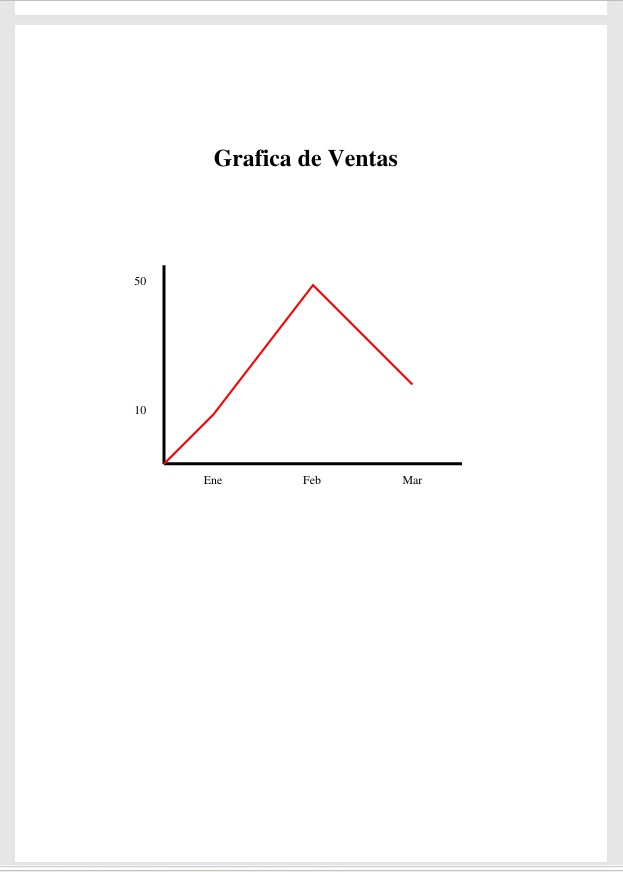
\includegraphics[width=0.9\textwidth]{images/ejer5_pg2.jpg}
\caption{Propuesta ejercicio 5. Página 2.}
\label{fig:5ejer2}
\end{figure}

El programa completo se puede ver en el anexo \ref{anexo:ej5}. En el anexo \ref{anexo:pdf5} se puede ver la página pdf generada.